\documentclass[onecolumn, oneside, a4paper, 11pt]{memoir}


\usepackage[utf8]{inputenc}
\usepackage[T1]{fontenc}

% Paths
\newcommand{\figs}{../figs}
\newcommand{\data}{../data}

% Fonts
\usepackage{newpxtext,newpxmath}
\renewcommand*\sfdefault{cmss}

% Units
\usepackage[detect-weight=true, binary-units=true]{siunitx}
\DeclareSIUnit\flop{Flops}

% Math
\let\openbox\undefined
\usepackage{amsthm}
\usepackage{amsmath}
\usepackage{amssymb}
\usepackage{bm}

\theoremstyle{remark}
\newtheorem{ex}{Exercise}
\newtheorem*{sol}{Solution}

% Graphics
\usepackage{graphicx}
\usepackage{caption}
\usepackage{subcaption}
\graphicspath{{../figs/}}

% Tikz
\usepackage{tikz}
\usetikzlibrary{positioning,shapes,arrows,calc,intersections}
\usepackage{pgfplots}
\usepgfplotslibrary{dateplot}
\pgfplotsset{compat=1.8}

% Colors
\definecolor{darkblue}{HTML}{00688B}
\definecolor{darkgreen}{HTML}{6E8B3D}
\definecolor{cadet}{HTML}{DAE1FF}
\definecolor{salmon}{HTML}{FFB08A}

% Listings
\usepackage{textcomp}
\usepackage{listings}
\lstset{
  keywordstyle=\bfseries\color{orange},
  stringstyle=\color{darkblue!80},
  commentstyle=\color{darkblue!80},
  showstringspaces=false,
  basicstyle=\ttfamily,
  upquote=true,
}
\lstdefinestyle{fortran}{
  language=Fortran,
  morekeywords={for},
  deletekeywords={status},
}
\lstdefinestyle{c}{
  language=C,
  morekeywords={include},
}
\lstdefinestyle{shell}{
  language=bash,
}

\begin{document}

\pagestyle{empty}

\begin{center}
  {\Huge \bfseries \scshape
    Introduction to \\[0.2\baselineskip] Supercomputing} \\[2\baselineskip]
  {\Large TMA4280 $\cdot$ Introduction to development tools} \\[2\baselineskip]
\end{center}

\section{Development tools}

During this course, only the \texttt{make} tool, compilers, and the GIT tool will be used for the sake of simplicity: no integrated development environment is required.
The purpose of the computers labs and project is to get you to do fairly low-level programming with C/C++ or FORTRAN using OpenMP and MPI. You need to be able to write simple algorithms involving vectors and matrice, manage the allocation/deallocation of memory, and compile/run the code.
Of course you are free to explore more advanced aspects of the development of numerical algorithms on a computer, feel free to ask questions.


\subsection{Revision control system}

In this section, we will use the \texttt{GIT} revision control system tool to create a local repository and push it to Github.
You need to create an account on GitHub to be able to create source code repositories.
Although, not crucial for this course, it will make your work more efficient and ease working with your teammate(s) on the projects.

\subsubsection{Motivations and goals}

The rationale behind Revision Control Systems (RCS) is that the history of code development should be kept to understand the evolution of the software, and that several individuals should be able to work on the same code base simultaneously.
Different RCS exist and adopt a more or less distributed collaborative approach.
GIT has become the most popular in the recent years (mainly because it is used by GNU/Linux communities), and offers a distributed environment for collaborating on projects.

\medskip
A collection of files can be \textit{tracked} using a RCS: the history of modifications of each file is recorded and can be reviewed at any time.
The collection of files \textit{tracked} and the metadata used to do so consist of a \textit{repository}.
In your case, the files will be source code, makefiles, reports, \dots
Whenever the collection of files tracked contains source code, it is usually called a \textit{source repository}.

\bigskip
\textbf{Concepts}

\medskip
The \textit{source repository} consists of a tree of directories containing the files (source code, build tools, documentation), \dots)
The history of changes to this collection of files will be kept and represented as a sequence of \textit{changesets}: any \textit{changeset} contains the modification to the files.
A new \textit{changeset} is created any time, you \textit{commit} the modifications.

\medskip
To allow simulaneous work on the code, the notion of \textit{branch} should be introduced.
You can represent working on a project with a \textit{tree}: the work is added to a reference version sometimes called a \textit{trunk}, but people should be able to work independently and simulaneously on the project, so they are able to create a local \textit{branch} containing their modifications.
Usually for software taska requiring modifications fall in the ``bug fix'' or ``feature'' category.
Sometimes the reference version changes and the \textit{local branch} needs be synchronized with a \textit{remote branch}.
When the task is completed, the \textit{local branch} can be synchronized with the \textit{remote branch}, possible conflicts solved (modifications to the same file), and finally merged.

\begin{center}
    \scalebox{0.8}{
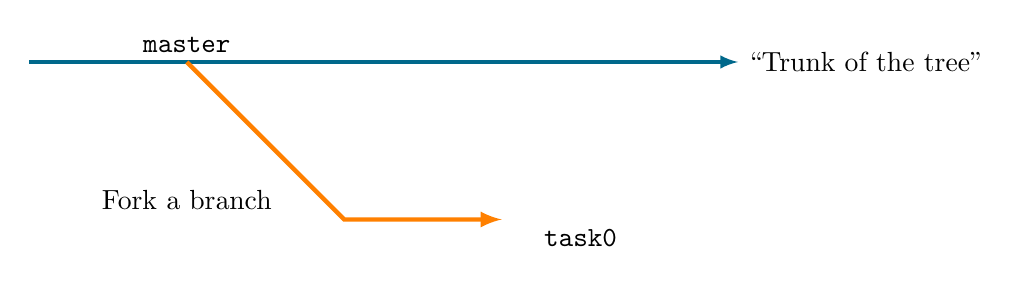
\begin{tikzpicture}
  \node[anchor=south] at (2,-1) {\texttt{master}};
  \draw[darkblue, very thick, -latex] (0,-1) -- (9,-1);
  \node[anchor=west] at (9,-1) {``Trunk of the tree''};
  \node[anchor=south] at (2,-3) {Fork a branch};
  \draw[orange, ultra thick, -latex] (2,-1) -- (4,-3) -- (6,-3);
  \node[anchor=north] at (7,-3) {\texttt{task0}};
\end{tikzpicture}
}
\end{center}

By default, a \textit{branch} name \texttt{master} is created: you can create a new branch from \texttt{master} to work on your own version of the code, then merge the modifications at a later stage.

\begin{center}
    \scalebox{0.8}{
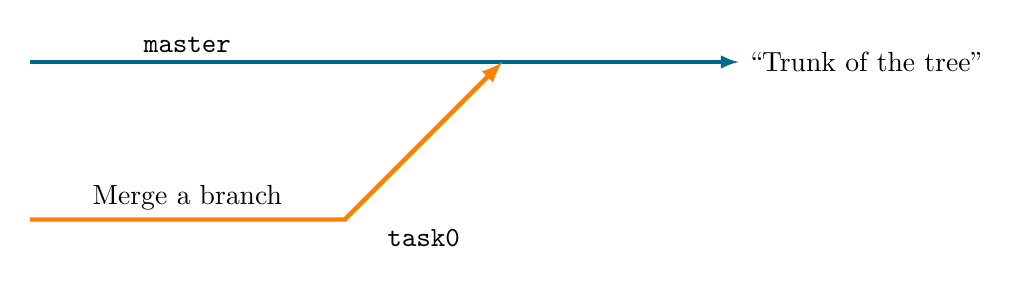
\begin{tikzpicture}
  \node[anchor=south] at (2,-1) {\texttt{master}};
  \draw[darkblue, very thick, -latex] (0,-1) -- (9,-1);
  \node[anchor=west] at (9,-1) {``Trunk of the tree''};
  \node[anchor=south] at (2,-3) {Merge a branch};
  \draw[orange, ultra thick, -latex] (0,-3) -- (4,-3) -- (6,-1);
  \node[anchor=north] at (5,-3) {\texttt{task0}};
\end{tikzpicture}
}
\end{center}

The workflow can be summarized as:
\begin{enumerate}
\item Fork a branch
\item Add modifications and synchronize if necessary
\item Solve conflicts
\item Merge
\end{enumerate}
The merge step on GitHub is performed using a ``Pull Request'': an issue is opened, the code is subject to review, and finally merged if approved.

\begin{ex}
Open a terminal and go to the directory you created last week, it does not contain a GIT repository yet:
\small{
\begin{lstlisting}[style=shell]
$ git status
fatal: Not a git repository (or any parent up to mount point /home)
Stopping at filesystem boundary (GIT_DISCOVERY_ACROSS_FILESYSTEM not set).
\end{lstlisting}
}

\bigskip
Follow the steps:
\begin{enumerate}
\item Use \texttt{git init} to create a local repository in this directory: you should see now a \texttt{.git} directory appear, do not delete it!
\small{
\begin{lstlisting}[style=shell]
$ git init
Initialized empty Git repository in /home/<user>/TMA4280/.git/
\end{lstlisting}
}

\medskip
\item Use \texttt{git status} to list files in the directory: they should be shown as \textit{untracked}.
\small{
\begin{lstlisting}[style=shell]
$ git status
On branch master

Initial commit

Untracked files:
  (use "git add <file>..." to include in what will be committed)

	README
	cat/
	shell/

nothing added to commit but untracked files present (use "git add" to track)
\end{lstlisting}
}
\medskip
\item Create an empty file named \texttt{README} and add it to the repository
\small{
\begin{lstlisting}[style=shell]
$ git add README 
$ git status
On branch master

Initial commit

Changes to be committed:
  (use "git rm --cached <file>..." to unstage)

	new file:   README

Untracked files:
  (use "git add <file>..." to include in what will be committed)

	cat/
	shell/
\end{lstlisting}
}
\item Create your first commit containing the README file (you can write your name in this file for example).
\small{
\begin{lstlisting}[style=shell]
$ git commit -m "Initial commit"
[master (root-commit) 4a177e4] Initial commit
 1 file changed, 1 insertion(+)
 create mode 100644 README
\end{lstlisting}
}
\medskip
\item Add all the files you created in the project directory \texttt{TMA4280} and commit them.

\item Create an account on GitHub then create a repository named \texttt{TMA4280v2018} in the user interface: this remote \textit{repository} will contain your files.

\item Follow the instruction on GitHub and upload (\texttt{push}) the local branch to the remote repository.
\small{
\begin{lstlisting}[style=shell]
$ git remote add origin https://github.com/<username>/TMA4280v2018.git
$ git push -u origin master
\end{lstlisting}
}
\end{enumerate}
\end{ex}

\bigskip
Now that your remote repository is created and updated with your initial files, let us have a quick look at the local repository.

\medskip

\begin{ex}
To understand the principle of commits and branches, follow the steps:
\begin{enumerate}
\item Use \texttt{git log} to look at the history of your repository.
\item Use \texttt{git branch} to list local branches.
\item Use \texttt{git checkout -b} to create a branch named \texttt{lab01} and list again the branches.
\item Use \texttt{git push} to push the branch to the remote repository and check on GitHub that it is listed.
\end{enumerate}
\end{ex}

\bigskip
With this simple introduction you should be able to manage the exercises and projects without risking losing your work.

\newpage
\subsection{GIT Reference}

This list presents basic actions that you may need to perform for managing your projects.

\textbf{Initialize a repository}

\begin{lstlisting}[style=shell]
git init
\end{lstlisting}

\textbf{Clone a repository}
\begin{lstlisting}[style=shell]
git clone <repository_location>
\end{lstlisting}

\textbf{Create a branch}

\begin{lstlisting}[style=shell]
git checkout -b <branch_name>
\end{lstlisting}

\textbf{Checkout file from other branch if necessary}

\begin{lstlisting}[style=shell]
git checkout <branch_name> -- <paths>
\end{lstlisting}

\textbf{Synchronize feature branch with master}

\begin{lstlisting}[style=shell]
git checkout <my_branch_name>
git pull --rebase origin master
\end{lstlisting}

\textbf{Cleanup commit history before merge}

WARNING: Don't cleanup history if more than one person works on the branch!

Find the number of last commits to be reordered with:
\begin{lstlisting}[style=shell]
git log
\end{lstlisting}
Then:
\begin{lstlisting}[style=shell]
git rebase -i HEAD~n
\end{lstlisting}
with n the number of commits to be treated (until now nothing is modified), or until the commit with given hash.
\begin{lstlisting}[style=shell]
git rebase -i hash

Use the following commands to change to first keyword

# Commands:
#  p, pick = use commit
#  r, reword = use commit, but edit the commit message
#  e, edit = use commit, but stop for amending
#  s, squash = use commit, but meld into previous commit
#  f, fixup = like "squash", but discard this commit's log message
#  x, exec = run command (the rest of the line) using shell
\end{lstlisting}

Using squash ('s') merges commits together.

Possibly use this command to change the last commit message
\begin{lstlisting}[style=shell]
git commit --amend
\end{lstlisting}

\textbf{Cleanup master branch locally}

\begin{lstlisting}[style=shell]
git pull --rebase origin master
git reset --hard
\end{lstlisting}

\textbf{Fetch all the branches from the remotes}

\begin{lstlisting}[style=shell]
git fetch --all
\end{lstlisting}

\textbf{Pick specific commits from any branch}

\begin{lstlisting}[style=shell]
git cherry-pick <commit_hash>
\end{lstlisting}

\textbf{Remove untracked files from working directory}

\begin{lstlisting}[style=shell]
git clean -f -d 
\end{lstlisting}

\textbf{Adding a reference to a bug}

Add a keyword and the ID in the commit message, like:
\begin{lstlisting}[style=shell]
git commit -m "This is nice commit message"
\end{lstlisting}

\newpage
\section{C Programming}

\begin{table}[h!]
\centering
\caption{Data types}
\begin{tabular}{|c|l|}
  \hline
  Type & Description \\
  \hline
  \texttt{char} & Signed or unsigned integer stored on 8 bits, a \textit{byte}. \\
  \texttt{short} & Integer of a least 16-bit long. \\
  \texttt{int} & Integer of a least 16-bit long, usually 32-bit long. \\
  \texttt{long} & Integer of a least same size as \texttt{int}, usually 32-bit long. \\
  \texttt{float} & Single precision floating-point number of size 32 bits \\
  \texttt{double} & Double precision floating-point number of size 64 bits \\
  \hline
\end{tabular}
\end{table}
Integer types can be \texttt{signed} or \texttt{unsigned}.


\begin{table}[h!]
\centering
\caption{Control flow statements and loops}
\begin{tabular}{|c|l|}
  \hline
  Name & Description \\
  \hline
  \texttt{if \{ \textit{condition} \} ( \dots )} & Conditional. \\
  \texttt{if \{ \textit{condition} \} ( \dots ) else ( \dots ) } & Conditional. \\
  \texttt{for (\textit{pre};\textit{condition};\textit{post}) \{ \dots \}} & Loop. \\
  \texttt{while (\textit{condition}) \{ \dots \}} & Loop. \\
  \texttt{do \{ \dots \}} while (\textit{condition})  & Loop. \\
  \texttt{switch (\textit{variable}) \{ case \textit{value}: \textit{body}; break; \dots \}} & Switch between cases. \\
  \hline
\end{tabular}
\end{table}

\begin{ex}
Let us create our first program, the famous ``\texttt{Hello world!}'':
\begin{enumerate}
\item Go to the \texttt{progs} directory and create a \texttt{hello0} subdirectory.
\item Create a \texttt{main.c} file, implement a program printing \texttt{Hello world!} in \texttt{C} using the \texttt{printf} function.
\item Compile and execute it.
  \begin{itemize}
  \item The code consists of a single source file.
  \item The compilation and linking can be done in a single command. \\
\begin{lstlisting}[style=shell]
gcc -o hello hello.c
\end{lstlisting}
  \item We might want to turn on compiler optimizations. \\
\begin{lstlisting}[style=shell]
gcc -o hello hello.c -O2
\end{lstlisting}
  \item We might want to include debugging info. \\
\begin{lstlisting}[style=shell]
gcc -o hello hello.c -g
\end{lstlisting}
  \end{itemize}
\item Copy the directory to \texttt{hello1}, create a header and source file to separate the implementation from the main file: list the commands required to build the program and write a Makefile.
\begin{lstlisting}[style=shell]
gcc -c -o hello.o hello.c
gcc -c -o utils.o utils.c
gcc -o hello hello.o utils.o
\end{lstlisting}
\item Modify the program to print \texttt{Goodbye world!} depending on an input argument, then add support for a number of times the message should be printed using \texttt{int ntimes = atoi(argv[1]);} to convert the argument.
\item Copy the directory to \texttt{hello2}, modify the Makefile to create a static library and link.
  \begin{itemize}
  \item We first link the printing functions into a library
\begin{lstlisting}[style=shell]
gcc -c -o hello_utils.o hello_utils.c
gcc -c -o goodbye_utils.o goodbye_utils.c
ar r libutils.a hello_utils.o goodbye_utils.o
\end{lstlisting}
  \item Then we build the program.
\begin{lstlisting}[style=shell]
gcc -c -o main.o main.c
gcc -o hello main.o libutils.a
\end{lstlisting}
  \end{itemize}
\end{enumerate}
\end{ex}

\begin{table}[h!]
\caption{Main function}
\centering
  \begin{lstlisting}[style=c]
#include <stdio.h>

int main(int argc, char **argv)
{
  return 0;
}
  \end{lstlisting}
\end{table}

\bigskip
Three directories \texttt{hello0}, \texttt{hello1}, and \texttt{hello2} provided in the repository will show you how to use Makefiles. Makefile are recipes to build programs, designed to overcome two difficulties:
\begin{itemize}
\item Compiler commands and options vary across systems and depend on the programming language,
\item Binaries are created in three main stages: the source code is pre-processed (ex: \texttt{cpp}), then compiled into objects (ex: \texttt{cc}) and finally linked into a library or executable (ex: \texttt{ld}).
\end{itemize}

\subsection{Small programming exercises}

\begin{ex}
\textit{Data model}. Implement a C/C++ program that creates four integer variables $i0, i1, i2, i3$ of type \texttt{char}, \texttt{short}, \texttt{int}, \texttt{long} and two real variable $r0, r1$ of type \texttt{float}, \texttt{double}.
Using the functions \texttt{printf} and \texttt{sizeof()} to print the number of bytes used for each data type.
Compile the program in $32-$ and $64-$bit using the \texttt{-m32} and \texttt{-m64} options, and note the values in a file.
Which model is used in the $64-$bit case?
\end{ex}

\begin{ex}
\textit{Matrix-Vector product}.
  Implement a C/C++ program that computes $\bm y = \bm A \bm x$.
  \begin{align*}
    \bm A =
    \begin{pmatrix}
      0.3 & 0.4 & 0.3 \\
      0.7 & 0.1 & 0.2 \\
      0.5 & 0.5 & 0.0
    \end{pmatrix}, \qquad \bm x = \begin{pmatrix} 1.0 \\ 1.0 \\ 1.0 \end{pmatrix}.
  \end{align*}
Two versions possible.
\end{ex}

\begin{ex}
\textit{Vector sum}. Implement a C/C++ program that creates three real vectors $\bm x, \bm y, \bm z$, one real number $\alpha$ and computes $\bm z = \alpha \bm x + \bm y$ for given $\bm x$ and $\bm y$ (double-precision).
First use a fixed-size of $10$ then implement a version with dynamic size.
\end{ex}

\begin{ex}
\textit{Dot product}. Implement a C/C++ program that creates two real vectors $\bm x, \bm y \in \mathbb{R}^N$ and one real number $\alpha$ and computes $\alpha = \sum_{i=1}^{N} \bm x_i \bm y_i$ for given $\bm x$ and $\bm y$ (double-precision).
\end{ex}

\end{document}
